\documentclass[a4paper]{article}
\usepackage{amsmath,amsfonts,amsthm}
\usepackage{fullpage}
\usepackage{float}
\usepackage{color}
\usepackage{graphicx}
\begin{document}

\newtheorem{lem}{Lemma}
\newtheorem{prop}{Proposition}
\newtheorem{rem}{Remark}
\renewcommand{\a}{\mathbf{a}}
\renewcommand{\v}{\mathbf{v}}
\title{Multiscale Adaptive Representation of Signals}
\author{Cheng Tai}
\date{}
\maketitle
\abstract{Starting with dictionary learning, we want to address two issues that we consider important. One is the inefficiency of sparse coding used by most dictionary learning scheme to encode a new incoming signal; the other is the lack of a truly multi-scale representation.}
\tableofcontents
\newpage
{\color{red}
\section*{TO DO}
\begin{enumerate}
\item Make the usage of $\|\cdot \|_2$ and $\| \cdot \|_2^2$ consistent, in particular, can we systematically replace all $\| \cdot \|_2^2$ with $\|\cdot\|_2$?
\item Make precise the proposition of sampling.
\item Make precise in what sense the model results a representation.
\item Add statement of robustness and proof.
\item Change the numerical experiments to numericla illustrations, since the purpose is to demonstrate the potential effectiveness and properties of the proposed new representation. By no means do we want to demonstrate how this model is superior to other models. 
\end{enumerate}
}
\section{Overview of dictionary learning and wavelets}
It is now well acknowledged that sparse and redundant representations of data plays a key role in many signal processing areas. The ability to represent a signal as a sparse linear combination of a few atoms from a possibly redundant dictionary lies in the heart of many models in signal processing, such as image/audio compression, denoising, and some higher level tasks such as pattern recognition.

Over the years, many efforts have been put on designing dictionary with certain properties. There are two lines towards this objective.  One line can be loosely called the analytic dictionary, which assume the mathematical properties of the class of signals of interest, and develops optimal representations for that class of signals. Examples include: Fourier basis, wavelets, wavelet tight frames, curvelets, contourlets, etc. The second kind takes a different route, it doesn't make assumptions about the mathematical properties of the class of signals, and tries to learn the dictionaries from the data from scratch. Beginning with the seminal work of Olshausen and Field, the field of dictionary learning has seen many promising advances. 

Models of the first kind are characterized by mathematical formulation and implicit transformations whereas the advantage of models of the second kind is that they lead to state-of-the art results in many practical low level signal processing applications. 

Despite the elegance and success of this methodology, there are also some important short comings to it, these include:
\begin{itemize}
	\item Computational cost is high. For the signals of length $N$, the trained dictionary $A\in \mathbb{R}^{m\times N}$ is stored and used explicitly. Each multiplication of the form $Ax$ or $A^Ty$ requires $O(mN)$ operations. In comparison, the analytic dictionary approach, such as Fourier transform only takes $O(N\log N)$ operations, and one level of wavelet transform take only $O(N)$ operations. When plugged to applications, we have to solve a relatively complex sparse coding program, even in the fastest greedy algorithms, such as Matching Pursuit, the matrix multiplications are carried out several times. Thus, because the learned dictionary is unstructured, it is much less efficient compared to traditional transform methods.
	\item Restriction to low-dimensions. Because the learning procedure requires solving a relative complex non-convex optimization program, the signals that can be practically trained is restricted to low dimensions, typically, $n\leq 1000$ is a reasonable limit. That is also a reason that in image processing applications, most popular models only train dictionaries on small image patches. An attempt to go beyond the limit raises a series of problems, the need for an huge amount of training data and intolerable training time.
	\item Operating on a single scale. Dictionaries as obtained by the MOD and the K-SVD operate on signals at a single small scale. Past experience with wavelets has taught us that often times it is beneficial to process the signals at several scales, and operates on each scale differently. This is actually related to the previous shortcomings, since the dictionary atoms that can be trained is small in size, which does not allow much room for multiple scales. There are some attempts in training multi-scale dictionaries, but this direction has not been thoroughly explored.
	\item Artifacts. As the dictionary operates on image patches, in tasks such as image compression, the patch wise operation produces visually unpleasant block effects along the boarders of the patch. Post processing is often needed to remove these artifacts. 
\end{itemize}

A natural question is, can we devise a way to get the best of both worlds? It is the goal of this paper to propose a partial solution to this question. In particular, we want to address two issues: the inefficiency of sparse coding used by most dictionary learning scheme to encode a new incoming signal and lack of a truly multi-scale representation. We will devise a novel representation of image signals with some favorable properties, such as multi-scale, computationally efficient, and is adapted to the signals as dictionary learning does.

%\section{A First Attempt to Improve Computational Efficiency of Dictioanry Learning}
%There are two routes we can take to reach our goal. One starts from dictionary and the other from wavelet tight frames. A route which we will not detail but will ultimately lead us to the same goal is the following: start with image patches, instead of training unstructured dictionary, we train tight frames, this helps improving the computational efficiency in that we don't need to solve a sparse coding program any more, instead, just perform one matrix vector multiplications. Next, we make the dictionary convolutional, based on the premise that image patches are shift invariant at a certain scale. Then, we would reach at something similar to a one layer adaptive wavelet tight frame transform. 
\section{Single Scale Adaptive Wavelet Tight Frames}
As a first step of the plan, we plan to construct wavelet tight frames in a manner that is adapted to the given data. The resulting model will be a building block of the multi-layer structure developed in later sections.We begin with a brief review of existing construction of wavelet tight frames.

\subsection{Wavelet Tight Frames}
In this subsection, we give a very brief introduction to wavelet tight frames, for a detailed introduction to this subject, the readers may refer to [].

Let $\mathcal{H}$ be a Hilbert space, we are mainly concerned with the case when $\mathcal{H}=L_p(\mathbb{R}^d)$. a system $X\subset H$ is called a tight frames is
\[
	\|f\|_2^2 = \sum_{x\in X} |\langle f,x\rangle |^2, \quad \textrm{for any } f\in \mathcal{H}
\]
There are two operators that are associated with a tight frame, one is the analysis operator defined as
\[
	W: f\in \mathcal{H} \rightarrow \{\langle x,f\rangle\}_{x\in X} \in l_2(\mathbb{N})
\]
and the other is the synthesis operator $W^T$, which is the adjoint operator of the analysis operator defined as
\[
	W^T : \{a_n\} \in l_2(\mathbb{N}) \rightarrow \sum_{x\in X} a_n x\in \mathcal{H}.
\]
The system $X$ is called a tight frame if and only if $W^TW=I$, where $I: \mathcal{H} \rightarrow \mathcal{H}$ is the identity operator. In other words, given a tight frame $X$, we have the following canonical expansion:
\[
	f=\sum_{x\in X} \langle x,f\rangle x, \quad \textrm{for any } f\in \mathcal{H}
\]
The sequence $Wf:=\{\langle f,x\rangle \}_{x\in X}$ are called the canonical tight frame coefficients. Thus, tight frames are often viewed as generalizations of orthonormal basis. In fact, a tight frame $X$ is an orthonormal basis for $\mathcal{H}$ if and only if $\|x\|=1,\forall x\in X$.

In signal processing applications, one widely used class of tight frames is the wavelet tight frames. The construction starts with a finite set of generators $\Psi:=\{\psi^1,\cdots,\psi^m\}$. Then consider the affine system defined by the shifts and dilations of the generators:
\[
	X(\Psi)=\{M^{j/2}\psi^{l}(M^j\cdot -k),1\leq l\leq m, j,k\in\mathbb{Z}, M\in\mathbb{Z^+}\}.
\]
The affine system $X(\Psi)$ is called a wavelet tight frame if it is a tight frame satisfying
\[
	f=\sum_{x\in X(\Psi)} \langle f,x\rangle x, \forall f \in \mathcal{H}.
\]
Wavelet tight frames used in practice are usually constructed from multi-resolution analysis(MRA). This is because a MRA structure is crucial for fast decomposition and reconstruction algorithms.  The MRA construction usually starts with a compactly supported scaling function $\phi$ with a refinement mask  $a_0$ satisfying
\[
	\hat{\phi}(M\cdot)=\hat{a_0}\hat{\phi}.
\]
where $\hat{\phi}$ is the Fourier transform of $\phi$, and $\hat{a_0}$ is the discrete Fourier series defined as $\hat{a_0}(\omega):=\sum_{k\in\mathbb{Z}} a_0(k) e^{-ik\omega}$ and $\hat{a_0}(0)=1$. After obtaining the scaling function, the next step step is to find an appropriate set of filters $\{a_1,\cdots,a_m\}$ and define the set of functions called framelets $\Psi=\{\psi_1,\cdots,\psi_m\}$ by
\[
	\hat{\psi_i}(M\cdot) = \hat{a_i}\hat{\phi},i=1,\cdots,m
\]
such that the affine system $X(\Psi)$ forms a wavelet tight frame. It is natural to ask when does such a system form a wavelet tight frame. Sufficient and necessary conditions are given by the so called Unitary Extension Principle(UEP). There are different versions of UEP principles, we are only concerned with one version that is associated with discrete wavelet tight frames, which we will state after a description of the decomposition and reconstruction operations. For a survey of UEP, the reader may refer to[].

Given a filter $a\in l_2(\mathbb{Z})$, the discrete decomposition and reconstruction transform are defined in the following way. Define the one dimensional down-sampling and up-sampling operator:
\[
	\begin{aligned}
		&[v\downarrow M](n):=v(Mn),\quad n\in \mathbb{Z}\\
		&[v\uparrow](Mn):=v(n), \quad n\in \mathbb{Z}
	\end{aligned}
\]
where $M$ a positive integer denoting the down-sampling or up-sampling factor. Down-sampling and up-sampling operators in higher dimensions are carried out by performing one dimensional operators along each dimension. 

Define the linear convolution operator $S_a: l_2(\mathbb{Z}) \rightarrow l_2(\mathbb{Z})$ by 
\[
[S_a(v](n):=[a*v](n)=\sum_{k\in\mathbb{Z}} (a(-\cdot)*v \downarrow)M, \forall v\in l_2(\mathbb{Z})
\]
For a set of filters $\{a_i\}_{i=1}^m\subset l_2(\mathbb{Z})$, we define its analysis operator $W$ by 
\[
	W=[S_{a_1(-\cdot)},S_{a_2(-\cdot)},\cdots,S_{a_m(-\cdot)}]^T.
\]
Its synthesis operator is defined as the transpose of $W$:
\[
	W^T=[S_{a_1(\cdot)},S_{a_2(\cdot)},\cdots, S_{a_m(\cdot )}].
\]
Now we may state the UEP for this situation.
\begin{prop}[cite]
Let $a_1,\cdots,a_m$ be finitely supported filters, the following are equivalent:
\begin{enumerate}
\item $W_a^T W_a = I$
\item for all $\omega \in [0,1)^d\cup M^{-1}\mathbb{Z}^d$,
	\[
		\sum_{i=1}^m \hat{a_i}\overline{\hat{a_i}(\xi + 2\pi\omega})=\delta(\omega);
	\]
\item for  all $k,\gamma \in \mathbb{Z}^d$,
	\[
		\sum_{i=1}^m \sum_{n\in\mathbb{Z}^d} \overline{a_i(k+Mn+\gamma)}a_i(Mn+\gamma)=M^{-d}\delta(k).
	\]
\end{enumerate}
\end{prop}
In particular, if the data are real numbers and no down-sampling is performed, then $W^TW=I$ is equivalent to 
\begin{equation}
\label{eq:uep}
	\sum_{i=1}^m \sum_{n\in \mathbb{Z}^d} a_i(k+n) a_i(n)=\delta_k, \forall k\in \mathbb{Z}^d.
\end{equation}
The linear B-spline wavelet tight frame used in many image restoration tasks is constructed via the UEP. Its associated tree filters are :
\[
	a_1=\frac{1}{4}(1,2,1)^T; \quad a_2=\frac{\sqrt{2}}{4}(1,0,-1)^T; \quad a_3=\frac{1}{4}(-1,2,-1)^T.
\]
Once the 1D filter $\{a_i\}_{i=1}^m$ for generating a tight frame for $l_2(\mathbb{Z})$ is constructed, the traditional way of generating higher dimensional tight frames is to use tensor products of 1D filters. But in this paper, we are going to construct 2D filters directly.

\subsection{Adaptive Construction}
We use shift-invariant systems because we accept the premise that at a proper scale, the statistical properties of image patches are translational invariant. Let $W_a$ be the matrix form of the analysis operator generated by the filters $\{a_i\}_{i=1}^m$, and let $W^T_a$ be the matrix form of the synthesis operator. Define $\mathcal{C}$ to be the set of filters that satisfy the full UEP condition, that is $\mathcal{C}=\{ \{a_i\}_{i=1}^m : W_a^TW_a=I\}$. Sometimes in image processing tasks, we can tolerance a little bit of loss of information, so we also consider the filters that approximately satisfy the full UEP condition within error $\delta$, $\mathcal{C}_\delta = \{\{a_i\}_{i=1}^m : \|W_a^TW_a -I\|_*\leq \delta\}$, where $\| \cdot \|_*$ means the operator norm.

For a given class of images and a specific task at hand, there are infinitely many discrete wavelet tight frames to choose from. Although they all provide perfect reconstruction of the input signal, some of them may provide sparser representations than the rest. Therefore, we propose a model that provides the sparest representation of the class of signals at hand. That is, the filters we are looking for is the minimizer of the following optimization program:
\begin{equation}
	\begin{aligned}
		&\min_{a_1,\cdots,a_m} \sum_{i=1}^m\Phi(v_i) \\
		\textrm{subject to} \quad&v_i = a_i(-\cdot)*x,\quad i=1,\cdots,m\\
		 & \{a_i\}_{i=1}^m \in \mathcal{C} \\
	\end{aligned}
\end{equation}
where $\Phi(x;a_i)$ is a sparsity inducing function, it can be chosen as, for example, the $l_1$ norm or $l_0$ "norm" or the Huber loss. We will focus the $l_1$ norm in the numerical illustrations given later as we find it attractive in terms of quality. That is,
\begin{equation}
\label{model:m0}
	\begin{aligned}
		&\min_{a_1,\cdots,a_m} \sum_{i=1}^m \|v_i\|_1 \\
		\textrm{subject to} \quad&v_i = a_i(-\cdot)*x,\quad i=1,\cdots,m\\
		 & \{a_i\}_{i=1}^m \in \mathcal{C} \\
	\end{aligned}
\end{equation}
As this optimization program is not convex, a local minimum is we can hope at best. We have no guarantee of the global optimality of the solution. Surprisingly, the local minimum obtained by interior point method are of very good quality in numerical experiments.

In some image processing tasks, such as pattern recognition, a small deviation from the perfect reconstruction filters is allowed. In that case, we consider
\begin{equation}
\label{model:m1}
	\begin{aligned}
		&\min_{a_1,\cdots,a_m} \sum_{i=1}^m \|v_i\|_1 \\
		\textrm{subject to} \quad&v_i = a_i(-\cdot)*x,\quad i=1,\cdots,m\\
		 & \{a_i\}_{i=1}^m \in \mathcal{C_\delta} \\
	\end{aligned}
\end{equation}

In this case, we can get an approximate solution to this model by penalty method, in fact, we have the following proposition:
\begin{prop}
Let $\{a\}_{i=1}^m$ be the minimizer of \eqref{model:m0}, let $\{\hat{a}_i\}_{i=1}^m$ be the solution to the following program:
\begin{equation}
	\label{model:m2}
	\begin{aligned}
		&\min_{a_1,\cdots,a_m} \sum_{i=1}^m \|v_i\|_1 + \eta \sum_k (Tr(A^TA,k)-\delta_k)^2 \\
		\textrm{subject to} \quad &v_i = a_i(-\cdot)*x,\quad i=1,\cdots,m
	\end{aligned}
\end{equation}
Then, for sufficient large $\eta$, we can correct $\hat{a}$ to be a solution $a^*$ such that the infeasibility of $a^* \sim \mathcal{O}(1/\lambda^2)$ and $\|v^*\|_1 \leq \|v\|_1 + \mathcal{O}(1/\lambda)$.
\end{prop}
\begin{proof}
	For notation simplicity, concatenate $\{a\}_{i=1}^m$ to form a single vector $a$, and similarly for $\{\hat{a}\}_{i=1}^m$. Let $F(a):=\sum_{i}^{m} \|a_j(-\cdot)*x\|_1$ and $G(a):= \sum_k (Tr(A^TA,k)-\delta_k)^2 $. 
	As $\hat{a}$ is minimizer of \eqref{model:m2}, $ F(a)+\eta G(a) \geq F(\hat{a}) + \eta G(\hat{a})$. But $G(a)=0, G(\hat{a})\geq 0$, hence $F(\hat{a})\leq F(a)$ and $G(\hat{a}) \leq \frac{1}{\eta} (F(a)-F(\hat{a}))$. Since $F(a)$ is bounded, $G(\hat{a}) \sim \mathcal{O}(1/\eta)$ as $\eta\rightarrow\infty$. Now we have a solution $\hat{a}$ with infeasibility $\mathcal{O}(1/\eta)$. we correct it as follows: for sufficient large $\eta$, $G(\hat{a}+e)=G(\hat{a})+\nabla G(\hat{a})e + o(\|e\|_2)$. As $G(a)$ is continuously differentiable, let $G(\hat{a})+\nabla G(\hat{a})e =0$, we have $e=-(\nabla G(\hat{a}))^{\dagger} G(\hat{a})$ where the $\dagger$ means Moore-Penrose Pseudo inverse, which gives a solution to the linear equation with smallest $l_2$ norm. Let $\sigma_m$ be the smallest singular value of $\nabla G(\hat{a})$, then because of our choice of $e$, we have $\|e\|_2 \sim \mathcal{O}(\frac{1}{\sigma_m \eta})$ and $G(\hat{a}+e)\sim \mathcal{O}(1/\eta^2)$. Define $a^*=\hat{a}+e$. Therefore, $\|v^*\|_1 - \|v\|_1 =\sum_{j=1}^m (\|a^*_j(-\cdot)*x\|-\|a_j(-\cdot)*x\|_1\leq \sum_{j=1}^m (\|a^*_j(-\cdot)*x\|-\|\hat{a}_j(-\cdot)*x\|_1\leq Cm\|e\|_1\leq C\sqrt{mr}\|e\|_2\leq C\frac{\sqrt{mr}}{\sigma_m\eta}$.
	
		\end{proof}

\begin{rem}
	For the sole purpose of getting nearly perfect reconstruction filters, the second term in the above model can be replaced by the following sample reconstruction error:
\begin{equation}
	\begin{aligned}
		&\min_{a_1,\cdots,a_m} \sum_{i=1}^m \|v_i\|_1 + \eta \|y-\sum_i a_i*a_i(-\cdot)*y\|_2 \\
		\textrm{subject to} \quad &v_i = a_i(-\cdot)*x,\quad i=1,\cdots,m
	\end{aligned}
\end{equation}
where $y$ is a sufficient large signal with each entry sampled from, e.g., a normal distribution.
\end{rem}
Optimization program \eqref{model:m2} is relatively easier to solve, we call it the sampling version of model \eqref{model:m1}. In practice, $\eta$ is chosen based on our tolerance of deviation from perfection reconstruction filters. By letting $\eta$ goes to $\infty$, we recover \eqref{model:m1}.  An illustration of the filters obtained is shown in Figure 1.
\begin{figure}[h!]
    \centering
    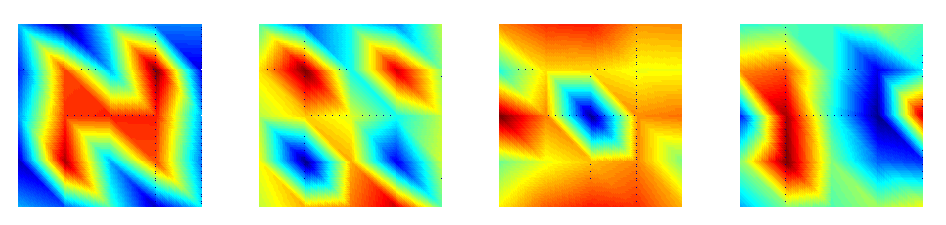
\includegraphics[width=0.5\textwidth]{fig11.eps}
  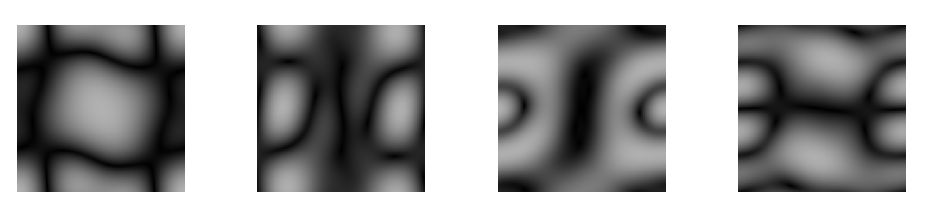
\includegraphics[width=0.5\textwidth]{fig12.eps}
    \caption{An examples of learned filters and their Fourier spectrum.}
    \label{fig:1}
\end{figure}

As numerical algorithms is not the focus of this paper, we omit the details of implementation here. A brief description of numerical algorithms is included in the appendix, numerical illustrations are reproducible through the MATLAB code online at []. 


So far, the models are based on the premise that the signals can be written as a sparse linear combination of translational invariant wavelets. Even if the signal is really generated this way, inevitably there will be perturbations or noises added to the coefficients. Hence, it is helpful to consider a variant of model \eqref{model:m1}:
\begin{equation}
\label{model:m3}
	\begin{aligned}
		&\min_{a_1,\cdots,a_m,v_1,\cdots,v_m} \sum_{i=1}^m \|v_i\|_1  + \lambda \sum_{i=1}^m \|v_i - a_i(-\cdot)*x\|_2^2\\
		\textrm{subject to} \quad& \{a_i\}_{i=1}^m \in \mathcal{C_\delta} \\		 
	\end{aligned}
\end{equation}
The sampling version can be written correspondingly.

The key feature of this variant, is that unlike the previous model, the wavelet coefficients $\{v_i\}$ is no longer linear dependent on $x$ given the filters $\{a_i\}_{i=1}^m$ yet still can be computed efficiently. Indeed, given the learned filters $\{a_i\}_{i=1}^m$ and the new input signal $x$, the coefficients is obtained by 
\[
	\min_{v_1,\cdots,v_m} \sum_{i=1}^m \|v_i\|_1 + \lambda \sum_{i=1}^m \|v_i - a_i(-\cdot)*x\|_2^2,
\]
the solution of which we can readily write explicitly:
\[
	v_i = \mathcal{T}_{1/2\lambda}( a_i(-\cdot)*x),\quad i=1,\cdots,m
\]
where $\mathcal{T}: \mathbb{R}\mapsto \mathbb{R}$ is the soft-thresholding operator defined by
\[
	\mathcal{T}_a(x)=\left\{ \begin{array}{lr}  (|x|-a)sign(x), &\textrm{ if } |x| > a \\0, &\textrm{otherwise}\end{array}\right . .
\]
When $\mathcal{T}$ operates on a vector, it operates on each component of the vector.


A special case of this variant, when the support of $a_i$ is of size $r\times r$ and $m=r^2$ and the filters are orthogonal to each other is proposed independently in [], and local solution is found by iteratively solving the $\{v_i\}_{i=1}^m$ and $\{a_i\}_{i=1}^m$.

To this end, we have introduced the construction of adaptive wavelet tight frames for one layer. When plugged into applications, we found the filters learned are of high quality, the results produced are comparable to those obtained by the dictionary learning paradigm, numerical illustrations are given in a later section, this is more or less expected.  In addition, we observed some quite unexpected and intriguing phenomena that we would like to share with the readers.
{\color{red} quadratic term needs to be verified}
\subsection{An Intriguing Phenomenon}
\textbf{A unique low frequency filter}. The most commonly used wavelets and wavelet tight frames constructed using MRA has only one low frequency filter. As a result, it enables a fast multi-level decomposition and reconstruction algorithm, the architecture is illustrated in Figure. However, the UEP does not distinguish between low frequency and high frequency filters, the concept of a unique low frequency  filter is more of mathematical considerations rather than practical need. Indeed, one need not be bounded by this restriction, and can use multiple low frequency filter. From a practitioner's point of view, as long as the filters provide sparse representations of the signal, we do not care much if there is one or multiple low frequency filters. Indeed, in proposing the previous models, we adopt this practitioner's point of view, hence no constraint on the number of low frequency filters is added in the models. One would expect the resulting filters would be of diverse frequencies.

Surprisingly, we found that, on many datasets, the filters learned contains exactly one low frequency filter. That is, among the $m$ filters trained, one and only one of them sums up to $1$, the rest each sum up to $0$ or very close to $0$, no intermediate values are presented. This phenomenon is stable regardless of the value of $m$ and support size of the filters. We observed this phenomenon on many datasets, including the Yale-face dataset, caltech-101 dataset, the fingerprint dataset, and a large number of randomly chosen natural photos from the Internet. However, this phenomenon is not entirely universal, we observed multiple low frequency filters on the dataset mnist. Apparently, this phenomenon has to do with the characteristics of the particular class of images and reflects the structure of the function space of all "natural images".A natural question is: for what class of images, can we observe such a phenomenon?

What this phenomenon means is that: the filters that give rise to the sparsest representation of image signals happen to have only one low frequency filter, which coincides with the traditional wavelets we have been using successfully in the past two decades. Some classes of images, exhibit sparse representations in these basis or tight frames, some don't. Notably, the majority the class of photos we conceptually take as "natural images" always exhibit such a phenomenon.(We haven't yet seen counter examples, but  Conversely, exhibiting this phenomenon can be thought of as a characteristic of the so called "natural images". 

\section{Extension to Mulitple Layers}
\subsection{Three Structures}
In this section, we introduce ways to extend the previous construction of adaptive wavelet tight frames to multiple layers. In going from one layer to multiple layers, we consider three typical structures which are conveniently illustrated in the following Figure.
\begin{center}
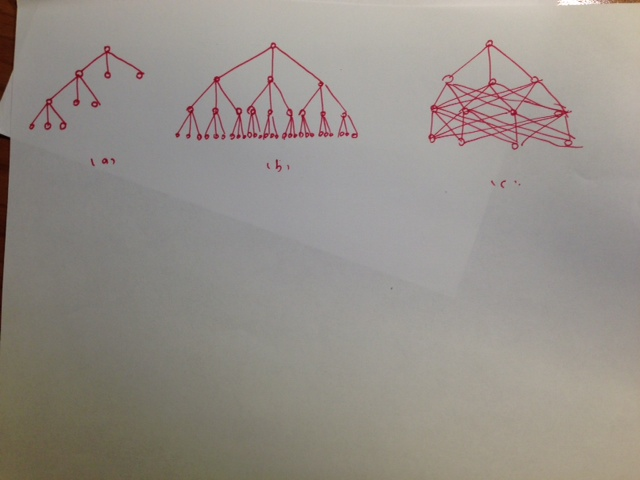
\includegraphics[scale=0.4]{arch.jpg}
\end{center}

The first structure is a partial $m-$tree, which corresponds to the multi-level wavelet or wavelet tight frame transform. The root node represents the input image, (for illustration purpose, the input image has only one channel), applying $m$ filters on the input, we get $m$ sets of wavelet tight frame coefficients. Each set of coefficients is represented using $m$-child nodes. The left most node always represents the low frequency coefficients. To do multi-level transform, we simply apply the same filters on the low frequency coefficients iteratively. Thus, for a level $L$ wavelet tight frame transform, the structure we get a tree of depth $L+1$ . 

This structure arises naturally in wavelet tight frames generated using MRA. The major advantage is the efficient decomposition and reconstruction algorithm. For level-$L$ transform with downsampling, it takes only $\mathcal O(mN)$ operations for the decomposition of a signal of length $N$.
 
Can we extend the previous adaptive construction to multiple levels using this structure? It depends. Such a structure assumes the existence of a single low frequency filter, which our previous construction does not guarantee. However, due to the pleasant surprise described in the previous section, for many datasets, we get a unique low frequency filter automatically. This phenomenon brings us a free lunch. It allows us to carry out multiple level transforms in exactly the same way as we do with pre-defined wavelet tight frames, only with improved performance. Our experience with numerical experiments suggests the rule of thumb, possibly exaggerated: {\color{red}wherever we have used wavelet tight frames for image processing tasks, we can try the adaptive construction using this structure. If we are lucky, we might improve the performance with no additional cost!} \\

The previous structure is great, but requires some luck. Sometimes we get a bunch of filters and no filter is more special than the others. This brings us to the second structure. The first layer is the same as the previous one. Below that, instead of doing transforms on the low frequency coefficients only, we do transforms on all sets of coefficients. As a result, the structure is a full $m$-tree. Apparently, the computational cost is now much larger. It is not appropriate for image compression or restoration tasks, but good for classification tasks. As the computational cost grows exponentially with the number of layers, we have to implement this structure with care and possibly some tricks in practice.  Examples of this structure include the scattering transform proposed by Mallat et.al. \\

It is the intention of creating a compact structure when we have no luck with the first structure that brings us to the third one. The first layer is still the same, below that, the tree structure is replaced by a fully connected structure. Because this structure is more elaborated and less known than the previous two, we shall give the details in the next subsection.

\subsection{The Proposed Multi-scale Structure}
The architecture consists an input layer and a few intermediate layers. The first layer is the same as the previous two structures, hence we focus on the intermediate layers. 

One intermediate layer accepts as input a few sets of coefficients produced by the previous layer, and produces another sets of output coefficients, not necessarily of the same number as the input. The input and output can be thought of as multi-channel images. The goal of the layer is still to produce sparse approximations of the input. Let $\{x_1,\cdots,x_m\}$ be the input coefficients, $\{v_1,\cdots,v_n\}$ be the output coefficients. The decomposition is defined as:
\begin{equation}
	v_j = \sum_i a_{ij}(-\cdot)*x_i,\quad j=1,\cdots,n
\end{equation}
and the reconstruction is defined as 
\begin{equation}
	x_i = \sum_j a_{ij}*v_j, \quad i=1,\cdots, m.
\end{equation}

Recognizing this as a 3D convolution, the UEP condition without downsampling then reads:
\begin{equation}
\label{uep:3d}
	\sum_{i=1}^m\sum_{j=1}^n  \sum_{n\in \mathbb{Z}^3} a_{ij}(k+n)a_{ij}(n) = \delta(k).
\end{equation}
We could explicitly incorporate this constraint and repeat what did in the previous sections. This amounts to solving
\begin{equation}
	\begin{aligned}
		&\min_{ \{a_{ij}\} } \sum_j \|v_j\|_1 \\
		\textrm{subject to} &\quad v_j = \sum_i a_{ij}(-\cdot)*x_i \\
			&\{a_{ij}\} \textrm{ satisfies \eqref{uep:3d}} \\
	\end{aligned}
\end{equation}
 But in practice, we find the resulting optimization program is not quite feasible to solve using a normal optimization procedure(It could be done though, just takes some time). Hence, we consider the following model based on the same sampling approximation spirit.
\begin{equation}
\label{eq:m3}
\begin{aligned}
	\min_{a_1,\cdots,a_m, v_1,\cdots,v_m}& \sum_i \|y_i - \sum_j a_{ij}*u_j\|_2 +\lambda \sum_j \|v_j\|_1 \\
	 \textrm{s.t.}  \quad v_j& = \sum_{i} a_{ij}(-\cdot)*x_i \\
		u_j&=\uparrow\downarrow(\sum_i a_{ij}(-\cdot)*y_i), \forall j.
	\end{aligned}
\end{equation}
The $\uparrow \downarrow$ represented a down-sampling followed by a up-sampling operation. It could be omitted if we are only interested in linear transform, however, the sampling operator need not be linear, it could be, for example max pooling and it reverse which are defined as 
\[
	\downarrow(c_1,\cdots,c_n) = (\arg\max_{c_1,\cdots,c_n} |c_i|, \arg\max_{i=1,\cdots,n} |c_i|)
\]
and its reverse
\[
	\uparrow(v,p)=(0,0,v,\cdots,0) \textrm{ with $v$ at the $p$-th location}.
\]
Unlike the linear sampling, in this case, we have to record both the value and position to get a reverse operation.

Similar to what did before, in the case where there is perturbation on the coefficients, we consider a particularly useful variant which we use in the numerical experiments.
\begin{equation}
\label{eq:m5}
\begin{aligned}
	\min_{\{a_{ij}\}, v_1,\cdots,v_m}& \sum_i \|y_i - \sum_j a_{ij}*u_j\|_2 +\lambda \sum_j \|v_j\|_1 + \eta \sum_j \|v_j-  \sum_{i} a_{ij}(-\cdot)*x_i \|_2^2\\
	 \textrm{s.t.}  	\quad 	u_j&=\uparrow\downarrow(\sum_i a_{ij}(-\cdot)*y_i), \forall j.
	\end{aligned}
\end{equation}
There is a subtlety considering stacking intermediate layer to form a multi-scale structures. That is, the output to input relation cannot be linear, otherwise stacking multiple layers would just be equivalent as a one layer structure. The non-linearity in our model may possibly come from two sources: one is the nonlinear sampling procedure, the other is the thresholding in the encoding stage.

Using \eqref{eq:m5} as a building block, we stack multiple layers together, we finally get the multi-scale structure depicted in Figure. The filters are all learned layer by layer, starting with the first one. Once the optimization has converged for the layer, we then move on to learn the next while keeping all filters in previous layers fixed.

\section{Properties of the Multi-scale Representation}
\subsection{From Approximation to Representation}
\subsection{Robustness}


\section{Numerical Illustrations}
In this section, we provide examples for the possible applications of the representation developed in the previous sections. Examples in image compression, denoising, classification will be given. 

\section{Discussions}
\subsection{Compare Dictionary Learning and Model A}
As we will see in this section, the dictionary learning models and model A share some similarities and have some differences. We make the following remarks: 

\textbf{1. Model A is convolutional form of dictionary learning.} Consider the training procedure of dictionary learning, given an image or a set of images, we collect all $r\times r$ non-overlapping patches and form them into a data matrix $X$, then we solve the following minimization program:
\begin{equation}
	\min_{D,C} \|X-DC\|_2^2 + \lambda\|C\|_1.
\end{equation}
The underlying rationale is at some scale, say $r$, the image patch can be approximated by a sparse combination of some basis functions, where each column of $D$ represents a base function and each column of $C$ represents the combination coefficients for a particular patch.
Consider model A in the one layer case, the objective function is 
\begin{equation}
\label{eq2}
	\min_{a_1,\cdots,a_m,v^{0}\cdots ,v^{m}} \|x-\sum_{i=1}^{m} a_i*v^{i}\|_2^2 +\lambda \sum_{i=1}^{m} \|v^{i}\|_1
\end{equation}
With some reorganization, this can be brought into a form that is very similar to dictionary learning. Let $X$ be the matrix formed by collecting all overlapping $r\times r$ images from an image, where each column of $X$ represents a vectorized image patch. Let $A=(vec(a_1),\cdots, vec(a_m))$, and $V$ is coefficient matrix which is reshaped conformally. Then the two terms in equation \eqref{eq2} are equivalent to :
\begin{equation}
	\min_{A,V} \|X-AV\|_2^2+\lambda \|V\|_1.
\end{equation}
This is exactly the same form as dictionary learning except for that in dictionary learning, the $X$ is formed from non-overlapping patches while in model A, $X$ is formed from overlapping patches. If we accept the premise that image patches are translation invariant at a certain small scale, then convolutional models are a natural choice. In fact, for the purpose of finding local basis, we could form $X$ by sampling randomly uniformly from the image. It should not be hard to show when the sample size is large, the resulted basis converges to the one obtained by solving \eqref{eq2}. The way dictionary learning forms the matrix $X$ corresponds to uniform sampling from a special non-lapping grid, hence a proper subset of all $r\times r$ image patches, which is unnatural. There are subsequent works on dictionary learning forming matrix $X$ by collecting two or more sets of non-overlapping image patches, which is more close to the translation invariance assumption.

Despite the formal similarities, there are usually striking difference between the two models in practice. For example, In the practice of training dictionary learning models, people often use very large number of dictionary atoms(256 or more), where as in convolutional bases, we only use a small number of basis function(usually no more than 32). The patch based reconstruction results visually unpleasant block effect, which needs to be removed by post processing, while model A does not have such an issue.(But critically sampled model may or may not suffer from block effect depending on the support of the filter.)

\textbf{2. Model A generalizes to multiple layers}. Being able to generalize to multiple layers of transform is crucial to a multi-scale representation. However, dictionary learning, in its original form, cannot achieve this objective. In dictionary learning, a dictionary is obtained and each image patch is associated with a few combination coefficients. As these coefficients are unordered and are of different length for different image patches, there is no obvious way how to continue learning the pattern of the coefficients in a similar "dictionary learning" fashion. In comparison, in model A, the coefficients associated with the image are still placed on a regular grid, which, after downsampling, are still of the same format as the input, which facilitates further learning in almost the same way. It is exactly this feature that allows model A to operates on multiple scales. 

\textbf{3. Computationally, the analysis based variant is favorable to dictionary learning}. When the parameters of both models are trained and to be used for inference, the computational costs are different. To infer the codes of a new incoming signal, dictionary learning performs a sparse coding, common procedures include matching pursuit, orthogonal matching pursuit and some path following algorithms, and they are of  different computational complexity. To solve model A in the synthesis formulation would require the same computation. However, there is an analysis based variant of model, which is far more efficient computationally in that it requires only a convolution plus a point-wise operation( such as thresholding). Compared with algorithms for solving sparse coding, there is a dramatic performance gain.

In this paper, we introduced a multi-scale adaptive representation of signals based on adaptive wavelet analysis. Demonstrations of possible applications are given to show the potential use of this tool. Obviously, there are some interesting questions remain unanswered: the phase transition as we increase the value of $\lambda$, for example. Due to the length constraint of this paper, we omitted several interesting aspects of the problem, for example, the robustness properties of the model to small deformations and translations.
{\color{red} Mallat's scattering transform is constructed using the second architecture, I wonder if the third construction also has the same robustness property, such as robust to translations and deformations?}


{\color{blue}
\subsection{Connections Between Three Models(with some conjectures)}
In this section, we establish some connections between the proposed model and the dictionary learning model, and auto-encoders. Much of this section is conjectured. I write them simply because I hope them to be true, although further investigations may prove them to be wrong. 

Given the signal $x$, we start with the model
\begin{equation}
	\begin{aligned}
		&\min_{v_1,\cdots,v_m,a_1,\cdots,a_m}& \sum_j \|v_j\|_1\\
		&\textrm{subject to} &\quad \|v_j - a_j(-\cdot)*x\|\leq \delta \\
		& &\{a_i\}_{i=1}^m \in \mathcal{C} \\
	\end{aligned}
\end{equation}

If we allow a small deviation from perfect reconstruction, we arrive at the model
\begin{equation}
	\begin{aligned}
		&\min_{v_1,\cdots,v_m,a_1,\cdots,a_m}& \sum_j \|v_j\|_1\\
		&\textrm{subject to} &\quad \|v_j - a_j(-\cdot)*x\|\leq \delta \\
		& &\{a_i\}_{i=1}^m \in \mathcal{C_\delta} \\
	\end{aligned}
\end{equation}

{\color{red} This model is equivalent to the following for an appropriate choice of $\lambda$}
\begin{equation}
	\begin{aligned}
		&\min_{v_1,\cdots,v_m,a_1,\cdots,a_m} \sum_j \|v_j\|_1 + \lambda \|y-\sum_j a_j*a_j(-\cdot)*y\|_2^2\\
		&\textrm{subject to} \quad \|v_j - a_j(-\cdot)*x\|\leq \delta \\
	\end{aligned}
\end{equation}
where $y$ is random gaussian variables.

If the input signal $x$ is sufficiently "rich", then the above model is equivalent to 
\begin{equation}
	\begin{aligned}
		&\min_{v_1,\cdots,v_m,a_1,\cdots,a_m} \sum_j \|v_j\|_1 + \lambda \|x-\sum_j a_j*v_j\|_2^2\\
		&\textrm{subject to} \quad \|v_j - a_j(-\cdot)*x\|\leq \delta \\
	\end{aligned}
\end{equation}

Apparently, if we drop the constraint that $\|v_j - a_j(-\cdot)*x\|\leq \delta$, we get back to the dictionary learning model, for a particular choice of $\lambda$. What difference does this make?

The original dictionary learning has too much freedom, as a result, we loses regularity. The decay of the coefficients obtained do not reflect the regularity of the signal. In the proposed model, the dictionary is always a tight frame, hence, not only doe it enable fast forward transforms but also the coefficients reflect the regularity of the signal. More importantly, because the coefficients are structured now, we can go up to build multiple layers, which is not the same if the coefficients are unstructured. If we are too greedy, we don't get to see the multi-scale structure.

The final model, formulated as an unconstrained problem, is the following:
\begin{equation}
	\begin{aligned}
		&\min_{v_1,\cdots,v_m,a_1,\cdots,a_m} \sum_j \|v_j\|_1 + \lambda \|y-\sum_j a_j*u_j\|_2^2 + \eta \|v_j - a_j(-\cdot)*x\|^2_2\\
	\end{aligned}
\end{equation}

Note in this formulation, the perfect reconstruction and the sparsity is separate, in the sparse coding setting, if we were to write a similar model, the minimization program would be:
\begin{equation}
	\begin{aligned}
		&\min_{v_1,\cdots,v_m,a_1,\cdots,a_m} \sum_j \|v_j\|_1 + \lambda \|x-\sum_j a_j*v_j\|_2^2 + \eta \|v_j - a_j(-\cdot)*x\|^2_2\\
	\end{aligned}
\end{equation}
But in our proposed model, the reconstruction term need not have anything to do with the input signal, it is a universal property. This would make the numerical scheme different, actually easier.

Next, consider the auto-encoder model. If the model is trained on a image patch instead of a whole image, then it can be well approximated by a convolutional form:
\begin{equation}
		\min_{a_1,\cdots,a_m}  \|x-\sum_j a_j*\sigma(a_j(-\cdot)x)\|_2
\end{equation}
Apparently, there is no sparsity promoting term here, we recognize if the $\sigma$ is the thresholding operator, then the minimizer of this program can be approximated by the proposed model with a prior other than sparsity.

The model is obviously equivalent to 
\begin{equation}
	\begin{aligned}
		&\min_{v_1,\cdots,v_m,a_1,\cdots,a_m} \|x-\sum_j a_j*v_j\|_2^2  \\
		\textrm{subject to} & \quad v_j =\sigma(a_j(-\cdot)*x)
	\end{aligned}
\end{equation}
but 
\[
	\sigma(y)=\arg\min_x \|y-x\|_2^2 + J(y)
\]
where $J(y)$ is a function shown in Figure .

In this case, the filter $a_i$ can never satisfy the perfect reconstruction unless the linear part of the $\sigma$ is used. The proposed model, with a different prior, can be compared against this one:
\begin{equation}
	\min_{v_1,\cdots,v_m,a_1,\cdots,_m} \|y-\sum_j a_j*a_j(-\cdot)u_j\|_2^2 + \lambda \sum_j J(v_j)+\|v_j-a_j(-\cdot)*x\|_2^2
\end{equation}

\subsection{Connection with convoluvional neural network}
The analysis based multi-scale structure resembles the deep convolutional neural networks even though we starts from a very different perspective, the wavelet tight frames. Despite the structure similarity, there are some striking difference between them. First, the convolutional neural network is a purely supervised learning machine, while the proposed model is unsupervised. Second, the proposed model is constructed with respect to the unitary extension principle, hence has the nearly perfect reconstruction property, whereas in deep convolutional neural networks, it is not clear how to reconstruct the input as much information is lost as we ascend the layers. In other words, the proposed model is a nearly lossless decomposition of the input signal, while the neural network is not.
}








\newpage
\section{Conclusion}
In this paper, we proposed a novel model that serve as a multi-scale adaptive representations of image signals. This representation improves over dictionary learning in two ways: the first is encoding efficiency, and the second is a truly multi-scale architecture. Numerical illustrations are given to show the potential effectiveness of this new representation. In addition, the new representation has the property of being robust to translations and deformations. Interesting connections between the proposed model and dictionary learning as well as auto-encoders are established and conjectured. 

Last but not least, this proposed model also leaves several interesting questions unanswered. For example, for what kind of dataset, is there a unique low frequency filter? How does this reflect the internal structure of function space of all "natural images"? Or should we do it conversely, "natural images" are characterized in part by the properties of the filters learned from it?

\section{Appendix}


















\end{document}